% #################################################
% Welcome to the LaTeX template file of Computer-Aided Design and Applications! 
% Please follow the instructions in this document to write and format your paper.
% We appreciate your submission. If you have any question, please feel free to 
% contact us at http://www.cadanda.com/Contactus.html.
% #################################################
\documentclass[9pt,academicons]{article}

\usepackage{CADA}
\usepackage{caption}
\usepackage{listings}
\usepackage{booktabs}       % professional-quality tables



% ####################################
% Add the title of your paper here. Each word is Capitalized! 
% ####################################
\title{MidcurveNN: Neural Network for Computing Midcurve of a Thin Polygon}


% #################################################
% This is where your paper begins. 
% #################################################
\begin{document}


% #################################################
% Sets up the beginning of the document (do not modify) 
% #################################################
\maketitle

% ############################################
% Here is the fun part. Please enter your:            
%      Name (First, Middle initial, Last)                  
%      Your ORCID number replace the "000-0000-1234-5678" part.    
% ############################################
\authorSection{
	\anAuthor{Yogesh H. Kulkarni}{0000-0001-5431-5727}{1}
}


% ######################################
% Here we need your affiliation and contact e-mail. Please edit   
% affiliation as well as the e-mail fields.                                  
% ######################################
\affiliationSection{
	\anAffiliation{1}{Pune, India}{yogeshkulkarni@yahoo.com}
}


% ######################################
% Please decide on who the corresponding author is going to be 
% and complete the section below                                            
% ######################################
\correspondingAuthor{Yogesh H. Kulkarni}{yogeshkulkarni@yahoo.com}


% ########################################
% Please type in your abstract below after the "\abstract{" part.
% ########################################
\abstract{Multiple applications demand lower-dimensional representation of geometric shapes. Midsurface is such a two-dimensional (2D) i.e., surface representation of a three-dimensional (3D) thin-walled solid shape. It is used in applications such as animation, shape matching, retrieval, finite element analysis, etc. Similarly, Midcurve is one-dimensional (1D) i.e., a curve representation of a two-dimensional (2D) sketch profile shape.  Methods available to compute Midcurves vary based on the type of the input shape (images, sketches, etc.) and processing (thinning, Medial Axis Transform (MAT), Chordal Axis Transform (CAT), Straight Skeletons, etc.). 
 
 
This paper talks about a novel method called MidcurveNN which uses Encoder-Decoder neural network for computing Midcurve from images of 2D thin polygons in a supervised learning manner. This dimension reduction transformation from input 2D thin polygon image to output 1D Midcurve image is learnt by the neural network, which can then be used to compute Midcurve of an unseen 2D thin polygonal shape.
}


% ########################################
% Please choose at least 3-5 good keywords and list them after the
% "\noindent \textbf{Keywords:}" part.
%
% The DOI part will be edited by us so please do not change that.
% ########################################
\keywords{Midcurve, Encoder-Decoder, Neural Network} 

\doi{10.14733/cadaps.2022.aaa-bbb}



%\noindent
%\textit{This template file was made up based on an actual paper written by Orest Mykhaskiv, Jens-Dominik M\"uller, Pavanakumar Mohanamuraly, Mladen Banovic, Andrea Walther, Salvatore Auriemma and Herve Legrand. The permission to use the paper is appreciated.}

% ################################
% You may now start your paper with an introduction
% ################################

\section{INTRODUCTION}
Computer-aided Design (CAD) models of thin-walled solids such as sheet metal or plastic parts are often reduced dimensionally to their corresponding Midsurfaces for quicker and fairly accurate results of Computer-aided Engineering (CAE) analysis (Figure~\ref{fig_cadcaeworkflow}).  

	\begin{figure} [!h]
		\centering
		\includegraphics[width=\linewidth,keepaspectratio]{images/Midcurve2}
		\caption{Computer-aided PDP (Source: Tierney\cite{Tierney2013})}
		\label{fig_cadcaeworkflow}
	\end{figure}
	



	\begin{figure} [!h]
		\centering
		\includegraphics[width=0.8\linewidth,keepaspectratio]{images/Midcurve5}
		\caption{Midsurface}
		\label{fig_midsurface}
	\end{figure}
	
A Midsurface is a surface lying midway of (and representing) the input shape (Figure~\ref{fig_midsurface}). Computation of the Midsurface is still a time-consuming and mostly, a manual task due to lack of robust-automated approaches. Many of the existing automatic Midsurface generation approaches result in some kind of failures such as gaps, missing patches, overlapping surfaces, etc. It takes hours or even days to correct such errors with manual intervention. Computing robust Midsurface, thus, is need of the hour.


	
%	\begin{figure} [!h]
%		\centering
%		\includegraphics[width=0.9\linewidth,keepaspectratio]{images/Midcurve13}
%		\caption{Midcurve}
%		\label{fig_Midcurve1}
%	\end{figure}
	
As Midsurface is 2D representation of a 3D thin solid, Skeleton (also known as Medial Object, Medial Axis, Chordal Axis, etc.) is one dimensional representation of either 3D or 2D input shapes. Various mathematical formulations/approaches used for their generation are Medial Axis Transform (MAT), Chordal Axis Transform (CAT), Pairing, Thinning, etc. (Figure~\ref{fig_medialmethods}). 

    \begin{center}
	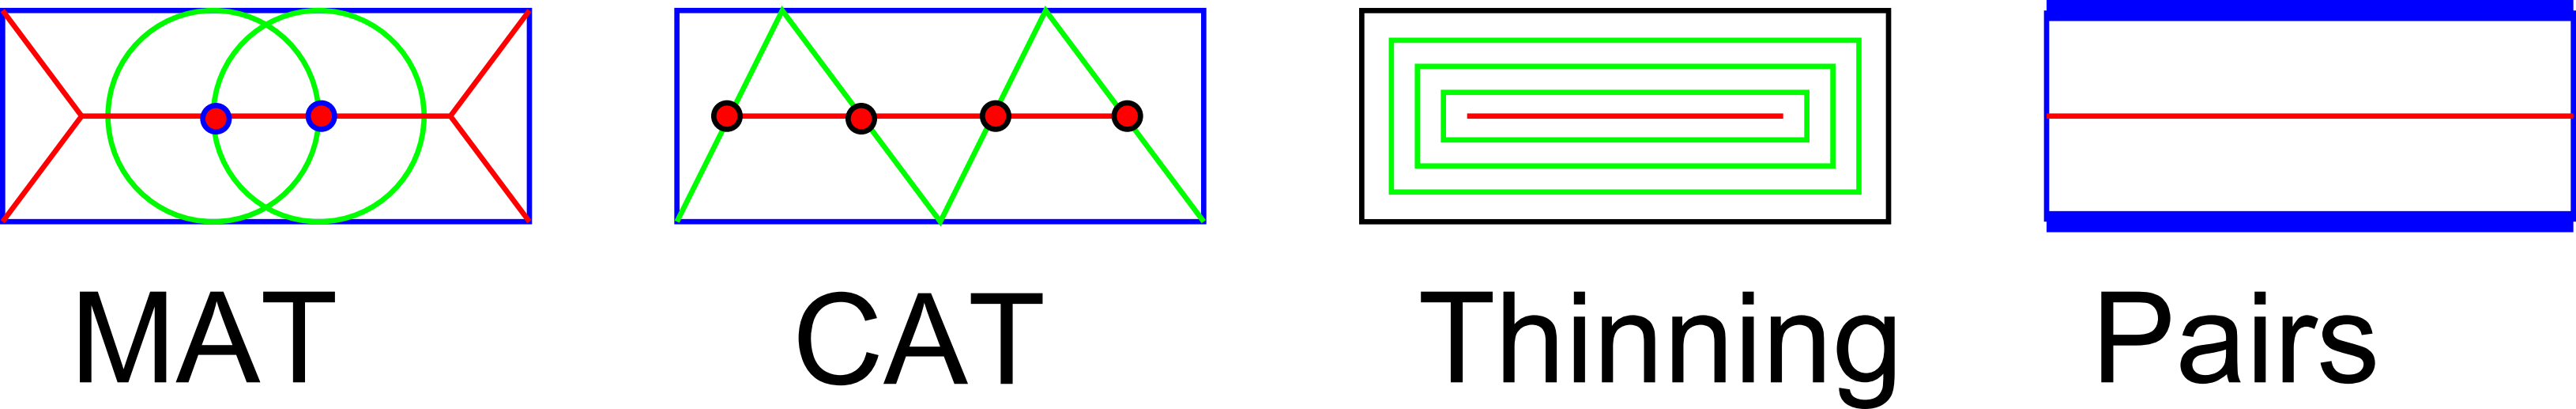
\includegraphics[width=0.6\linewidth]{images/MedialMethodsOnlyShort}
	\captionof{figure}{Medial Object computation methods}
	\label{fig_medialmethods}
    \end{center}
		
Midcurve is a special case of the Skeleton or MAT (Figure~\ref{fig_Midcurve1}) where the input shape is a 2D profile. Figure~\ref{fig_midmat} shows that Midcurve lacks the branches and morphologically represents the input shape \cite{Ramanathan04}. MAT and the input shape are dual (i.e. inter-convertible) whereas Midcurve does not have that requirement.

{\bf Definition:} \textit{Midcurve is an aggregation of curve segments (where each segment corresponds to a pair of nonadjacent edges in the object that are closest to each other) that form a closed and connected set and that satisfy homotopy}


    \begin{center}
	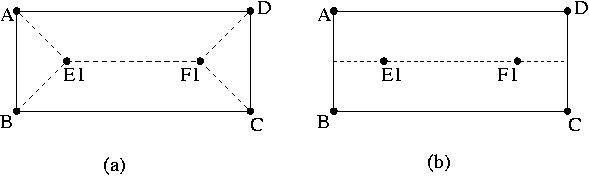
\includegraphics[width=0.5\linewidth]{images/Medial-Axis-and-Mid-curve_W640}
	\captionof{figure}{Medial Axis Transform (MAT) and Midcurve. \cite{Ramanathan04}}
	\label{fig_midmat}
    \end{center}
		
In CAD, thin solid shapes are typically created by extruding 2D sketch profiles. Thus, generating Midsurface is same as extruding Midcurve of the profile (Figure~\ref{fig_Midcurve}).

	\begin{figure} [!h]
		\centering
	\subfloat[]{\label{fig_Midcurve}\includegraphics[width=0.47\linewidth]{images/Midcurve12}} \quad
	\subfloat[]{\label{fig_Midcurve1}\includegraphics[width=0.47\linewidth]{images/Midcurve13}}
		\caption{Midcurve}
	\end{figure}
	
	
Midcurve, being simpler than the input shape, operations like pattern recognition, approximation, similarity estimation, collision detection, animation, matching and deformation can be performed efficiently on it rather than on the input shape. 



\section{RELATED WORK}

Research on computing Midsurface and Midcurve is going on for decades. Figure ~\ref{fig_litsurvey}) shows important milestones along the journey. More detailed analysis can be found in the survey paper \cite{medial2010}.

    \begin{center}
	\includegraphics[width=\linewidth]{images/Midcurve15}
	\captionof{figure}{Milestones along journey of Midsurface computation research}
	\label{fig_litsurvey}
    \end{center}
    

Following are some salient observations of these classical approaches:
\begin{itemize}[noitemsep,topsep=2pt,parsep=2pt,partopsep=2pt]
	\item Biggest strength of formal approaches like MAT is that it can be computed of any shape, thick or thin. Being formally defined, the converse or reversal process, meaning ``given a MAT compute the original shape'', is possible.
	\item Major drawback of MAT, Thinning methods is that it creates unnecessary branches and its shape is smaller than the original corresponding faces.
	\item  MAT based approaches also suffer from robustness problem. A slight change in base geometry forces re-computation of MAT and the results could very well be different than the original.
	\item Although MAT approaches have been around for decades and are fairly mature, its usage in Midcurve generation is still very complex and difficult to ensure appropriate topology.
	\item The major limitation of CAT approach is that mesh has to be generated beforehand. Creating constrained, single layer meshes on complicated 2D profiles are, at times, difficult.
	\item Thinning approaches are based on split events of the straight line skeleton gives counter-intuitive results if the polygon contains sharp reflex vertices.
	\item In Pairs approach, the two input curves or surfaces may not be in one-to-one form. In such cases maintaining continuity can be challenging.
	\item Quality of Midcurve generated by Pairs approach depends on the sampled input shape points.
\item Midcurve by profile decomposition approach is not used widely. The decomposition can result in large number of redundant sub-shapes making it ineffective and unstable for further processing.
\end{itemize}


The survey paper \cite{medial2010} suggests to avoid formal methods such as MAT, CAD, Thinning and Parametric, for computing Midcurve as they need heavy post-processing to remove unwanted curves. The heuristic method of decomposition,  has been error prone and inefficient so far. Author's own past work (Figure ~\ref{fig_Midcurveyk}) demonstrates reasonable success on simpler shapes, but being rule-based approach, had limitation on scalability.

    \begin{center}
	\includegraphics[width=\linewidth]{images/Midcurve16}
	\captionof{figure}{Midcurve Computation by Cellular Decomposition \cite{dimred2017}}
	\label{fig_Midcurveyk}
    \end{center}
    
%
%
%Many past approaches assume the input profile to be of simple polygon type, meaning, all the profile curves are linear and non-intersecting. The polygonal profile is assumed to be a set of connected lines end to end and closing the loop.
%
%Keil~\cite{Keil94} presented an approach based on convex partitioning, i.e. partitioning polygon at concave vertices, with an intent of making sub-polygons, convex. Figure~\ref{fig_keil} shows how his approach finds all possible ways to remove concavity of vertices and then takes the one that requires fewest diagonals.
%
%Lien et. al.~\cite{Lien2004} decomposed polygons 'approximately' based on iterative removal of the most significant non-convex feature. 
%
%Bayazit~\cite{Bayazit} presented a polygon decomposition method based on Concave (Reflex) angle partitioning. Figure~\ref{fig_bayazit} shows the partitioning at specific concave vertices. Although the output was far better than if usual meshing had been employed, the drawback was it left out some corner cases giving more than necessary divisions.
%
%%%\bigskip
%
%	\begin{figure}[!h]
%	\centering     %%% not \center
%	\subfloat[Keil~\cite{Keil94}]{\label{fig_keil}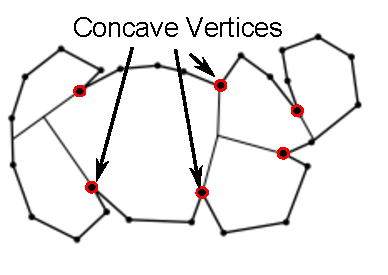
\includegraphics[width=0.4\linewidth]{images/keilwnames.pdf}} \quad
%	\subfloat[Bayazit~\cite{Bayazit}]{\label{fig_bayazit}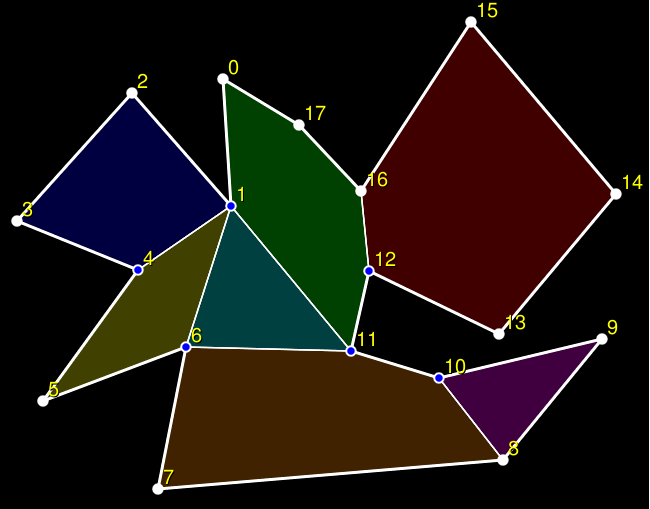
\includegraphics[width=0.4\linewidth]{images/bayazit}}
%	\caption{Polygon Decomposition Methods} %%%%%%%% ADD (\{citeYogeshIITG2014}) LATER
%	\label{fig:litsurvey:polydecomp}
%	\end{figure}
%	
%Rocha~\cite{Rocha98}~\cite{Rocha99} presented skeletonization approach for images which primarily worked on vertices. Figure~\ref{fig_rocha} shows how the sub-shapes computed mid-segments which were joined at the connections. Although this approach could address many shapes, it lacked comprehensive coverage and did not do very well for simple joints like T and L
%
%%%\bigskip
%
%\begin{figure}[h]
%\centering 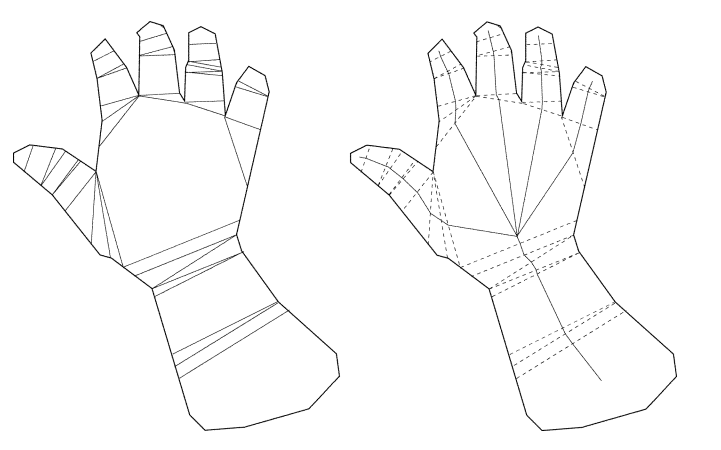
\includegraphics[width=0.5\linewidth]{images/rocha} 
%\caption{Midcurve Computation after Polygon Decomposition}
%\label{fig_rocha}
%\end{figure}

Use of Neural Network based techniques have been employed in recent times to compute Skeletons-Midcurve, primarily via image processing way. Rodas \cite{Rodas2019JointOB} used Deep Convolutional Neural Networks to compute object boundary as well as its skeletons, jointly. Shen et. al \cite{shen2016object,Shen_2017} built Convolutional neural network based skeleton extractor which is able to capture both local and non-local image context in order to determine the scale of each skeleton pixel. Zhao \cite{zhao2018hifi} used a similar method to \cite{shen2016object,Shen_2017} but introduced a hierarchical feature learning mechanism. Wang et. al.\cite{wang2018deepflux} introduced content flux in skeletons, which is
the learning objective instead of treating it as a binary classification problem. Approach by Panichev et. al. \cite{Panichev_2019_CVPR_Workshops} comes close to the method proposed here. It used U-net to extract skeletons, but not Midcurve though.
	
Review of the state-of-the-art suggests approaches for computing Midcurve are needed to take into account the application context, accuracy, characteristics  and aspect ratio of the sub-polygons. For the present research work, the Midcurve generation needs primitive shaped, thin sub-polygons. Non-primitive, skewed shapes would result in inappropriate Midcurves.

The current paper proposes a novel method of computing Midcurve using Neural Networks i.e Deep Learning approach.
 
 
\section{PROPOSED METHOD}
\label{sec:proposedmethod}

The current paper focuses on computing Midcurve for 2D planar sketch profiles and not 3D skeletonal shapes.  Even in 2D profiles, shapes vary enormously. As the first level of simplification, 2D polygons only (with an assumption that curved shapes can be converted to polygonal shape by faceting) are dealt with. Figure~\ref{fig_letters} shows some of the input shapes which can be considered. English alphabets are chosen for easy understanding and verification of the proposed method.

     \begin{center}
	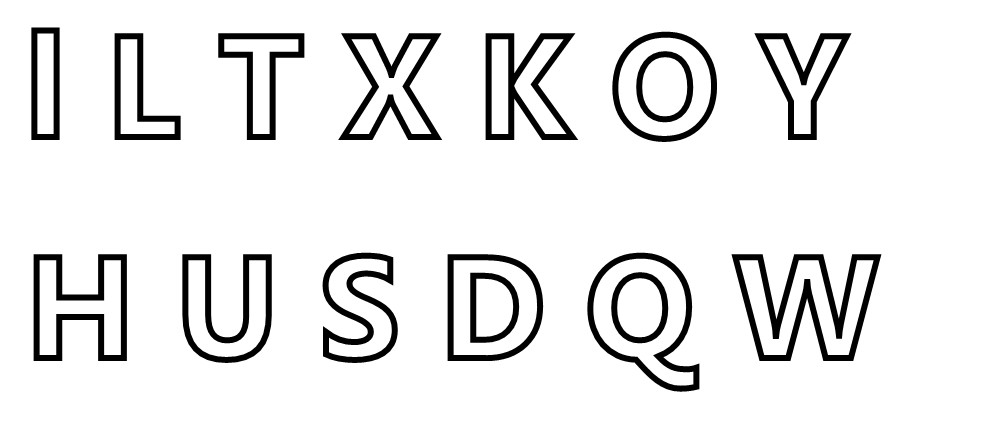
\includegraphics[width=0.9\linewidth]{images/Letters}
	\captionof{figure}{2D Thin Polygonal shapes}
	\label{fig_letters}
    \end{center}
		
		
Computation of Midcurve, in its original form, is transformation of a 2D thin closed, with/without-holes polygon to 1D open/closed/branched polyline. Paper \cite{dimred2017} details one of the effective Midcurve computation techniques, based on rule-based computational geometry approach. Such techniques have a shortcoming of not being scalable or generic enough to be able to handle variety of shapes. Deep Learning neural network architectures show potential of developing such generic models. This dimension reduction transformation should ideally be modeled as Sequence to Sequence (Seq2Seq) neural architecture, like Machine Translation. 

     \begin{center}
	\includegraphics[width=0.8\linewidth]{images/Midcurve_encoder_decoder}
	\captionof{figure}{Encoder-Decoder Architecture}
	\label{fig_endecoder}
    \end{center}
    
    
In the current problem, the input and the output sizes could be different not just in a single sample, but across all samples. Many current Seq2Seq neural networks need fixed size inputs and outputs, which if not present in data, are artificially managed by adding padding of certain improbable value. Such padding is not appropriate for the current Midcurve computation problem, as the padding-value can inappropriately get treated as part of the valid input. In this initial phase, to circumvent the problem of variable size, image-based inputs and outputs are used, which are of fixed size. Both input and output polygonal shapes are rasterized into images of 100x100, thus making them fixed size for all samples, irrespective of the original shapes.

This paper proposes to use such network for Midcurve computation in the form of image-to-image mode. Input images have thin polygonal shapes whereas output images have corresponding Midcurve images. Figure ~\ref{fig_endecoder} shows the Encoder-decoder architecture, called MidcurveNN.


    
Input and output geometries are rasterized into 100x100 size images. Transformations like translation, rotation and mirroring are applied to create diversity in the samples. MidcurveNN being a Supervised Learning approach, both input thin-polygons and corresponding output Midcurve polylines are transformed simultaneously. Figure~\ref{fig_training} shows some samples. This is training data.    


     \begin{center}
	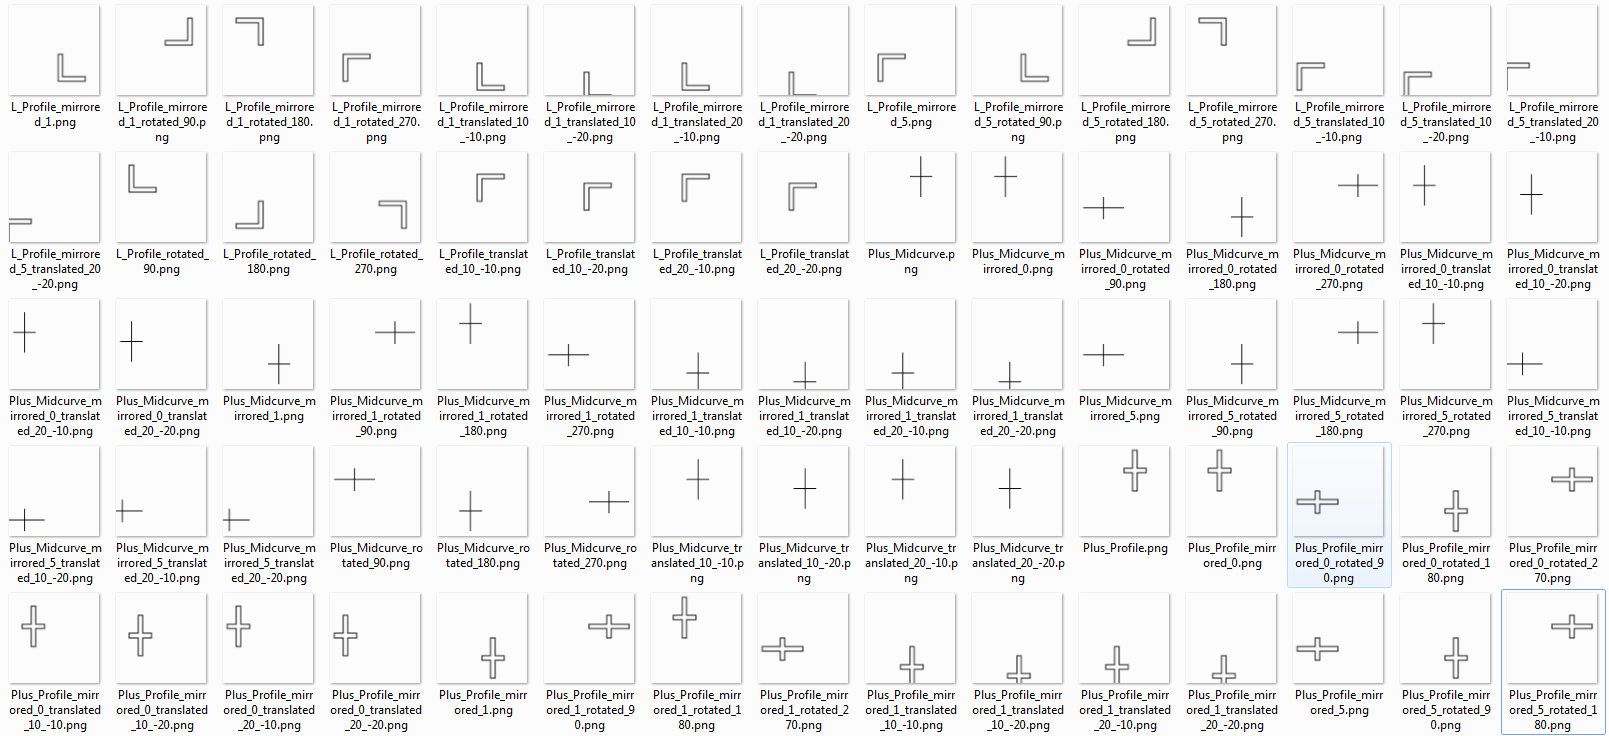
\includegraphics[width=\linewidth]{images/training_data}
	\captionof{figure}{Training Data: Inputs (thin polygons) and outputs (Midcurves)}
	\label{fig_training}
    \end{center}
    
MidcurveNN encoder-decoder has been implemented in Python programming with Keras library \cite{autoenkeras}.  

Abridged code listing is presented below (Code Listing ~\ref{lst:encdec}).

\begin{center}
\begin{tabular}{c}
\begin{lstlisting}[language=Python, caption=Encoder-Decoder,label={lst:encdec},frame=single]
input_img = Input(shape=(input_dim,))
    
encoded = Dense(encoding_dim, activation='relu')(input_img)
decoded = Dense(input_dim, activation='sigmoid')(encoded) 
    
autoencoder = Model(input_img, decoded)
            
encoder = Model(input_img, encoded)
encoded_input = Input(shape=(encoding_dim,))
decoder_layer = autoencoder.layers[-1]
decoder = Model(encoded_input, decoder_layer(encoded_input))
    
autoencoder.compile(optimizer='adadelta', loss='binary_crossentropy')
\end{lstlisting}	
\end{tabular}
\end{center}

Encoder takes input image of size $100 \times 100 = 10000$, then comes Dense layer with size $100$ to form the encoded vector. Decoder takes encoded vector as input, then with a Dense layer expands back to $100 \times 100 = 10000$ size of the output image. Relu activation is used for Encoder whereas Sigmoid for the decoder. AdaDelta optimizer with binary cross entropy as loss function is used to compute the losses. Table~\ref{tbl_loss} shows loss across number of epochs.    


\begin{table}[h]
\captionof{table}{Improvement in performance with epochs}
\centering

\begin{tabular}[htbp]{@{} p{0.14\linewidth}  p{0.22\linewidth}  p{0.22\linewidth}  @{}} \toprule
{\bf Epochs } & {\bf Training loss }  & {\bf Validation loss} \\
\midrule
50	& -17.6354	& -8.3223\\
200	& -16.8878	& -7.7672 \\
\bottomrule
\end{tabular}
\label{tbl_loss}
\end{table}


Some of the results are shown in Figure~\ref{fig_results}. Inputs are at the top and output Midcurve at the bottom.

     \begin{center}
	\includegraphics[width=\linewidth]{images/Midcurvenn_results}
	\captionof{figure}{Predicted Data: Inputs (thin polygons) and outputs (Midcurves)}
	\label{fig_results}
    \end{center}

Shape on the top is the input thin polygon whereas the corresponding shape at the bottom is the predicted Midcurve. It can be clearly seen that the network is able to localize the shape and learn the dimension reduction function reasonably well. It is still not perfect or usable, as some stray points are still being wrongly classified as the part of output Midcurve. A better network model and/or post processing is needed to make output Midcurve practically usable.


\section{CONCLUSIONS AND FUTURE WORK}

Traditional methods of computing Midcurves are predominantly rules-based and thus, have limitation of not developing a generic model which will accept any input shape. MidcurveNN, a novel Encoder-Decoder network attempts to build such a generic model. This paper demonstrates that simple single layer encoder and decoder network can learn the dimension reduction function reasonably well. Although more development is necessary in evolving a better neural architecture, the current results show positive potential. 

Working on truly variable size inputs (thin polygon) and outputs (polyline) using dynamic graph of Encoder-Decoder network can be attempted in the future. More and highly diversified data can help improve the quality of the output. Developing a formal representation of polygonal shapes with variations such as open/closed, with-without loops, branched as a coherent sequence of points is also on the agenda.

\bigskip
%\section*{ORCID}
\orcid{Yogesh H. Kulkarni}{0000-0001-5431-5727}
 

% #########################################
% Please pay close attention to the formatting of the references:
%    Authors: Smith, J.; Doe, M.; White, K.:
%    Paper: listed as published
%    Journal: listed in its conventional name
%    Volume: 27(3), 2009, 123-130, i.e. volume, issue, year and pages
%    Conference: name, location, year, pages
%    DOI: https://doi.org/DOI number. You can get the entire link from
%    "https://doi.crossref.org/simpleTextQuery/"
%    Books: author(s), title, publisher, location, year
%    Website: title (if any) and full URL link
% ##########################################

\referenceSection
\bibliographystyle{CADA}
\bibliography{CADandA_Paper_MidcurveNN}




\bigskip
\end{document}
